\documentclass[10pt,a4paper]{article}
\usepackage[a4paper,margin=1.8cm,top=1.6cm,bottom=1.7cm]{geometry}
\usepackage[T1]{fontenc}
\usepackage{cmbright}
\usepackage[default]{lato}
\usepackage{amsmath,amssymb}
\usepackage{graphicx}
\usepackage[dvipsnames,table]{xcolor}
\usepackage{booktabs,tabularx,array}
\usepackage[skins,breakable]{tcolorbox}
\usepackage{tikz}
\usetikzlibrary{shapes.geometric,arrows.meta,positioning,calc}
\usepackage{caption}
\usepackage{enumitem}
\usepackage{titlesec}
\usepackage{microtype}
\usepackage[colorlinks=true,linkcolor=cblue,urlcolor=cblue,citecolor=cblue]{hyperref}

\definecolor{cblue}{HTML}{1C86C8}
\definecolor{cgreen}{HTML}{2A9D4B}
\definecolor{corange}{HTML}{E8890C}
\definecolor{cred}{HTML}{D7263D}
\definecolor{cviolet}{HTML}{7B4FD0}
\definecolor{cpink}{HTML}{D6336C}
\definecolor{ctxt}{HTML}{1F2933}
\definecolor{cgray}{HTML}{6B7280}
\definecolor{cbg}{HTML}{F3F6FA}

\color{ctxt}
\setlength{\parindent}{0pt}
\setlength{\parskip}{4pt}
\linespread{1.04}
\captionsetup{font=small,labelfont={bf,color=cblue},skip=3pt,margin=0pt}
\setlist{itemsep=1pt,topsep=2pt,leftmargin=14pt}
\setlength{\abovedisplayskip}{4pt}\setlength{\belowdisplayskip}{4pt}
\setlength{\abovedisplayshortskip}{2pt}\setlength{\belowdisplayshortskip}{2pt}
\setlength{\textfloatsep}{8pt}\setlength{\floatsep}{6pt}\setlength{\intextsep}{6pt}

\titleformat{\section}{\large\bfseries\color{ctxt}}{\textcolor{cblue}{\thesection}}{0.6em}{}
\titlespacing*{\section}{0pt}{8pt}{3pt}
\titleformat{\subsection}{\normalsize\bfseries\color{ctxt}}{\textcolor{cblue}{\thesubsection}}{0.5em}{}
\titlespacing*{\subsection}{0pt}{5pt}{1pt}

\newtcolorbox{keybox}[2][cblue]{enhanced,colback=#1!6,colframe=#1,boxrule=0pt,leftrule=3pt,arc=1mm,
  left=6pt,right=6pt,top=3pt,bottom=3pt,fonttitle=\bfseries\small,coltitle=#1,
  title={#2},attach title to upper={\quad},before skip=4pt,after skip=4pt}
\newtcolorbox{numbox}[1][corange]{enhanced,colback=cbg,colframe=cbg,boxrule=0pt,leftrule=2pt,colframe=#1,arc=1mm,
  left=6pt,right=6pt,top=1pt,bottom=1pt,before skip=3pt,after skip=4pt}

\newcommand{\elastic}[1]{\textcolor{cblue}{#1}}
\newcommand{\plastic}[1]{\textcolor{corange}{#1}}
\newcommand{\MPa}{\,\mathrm{MPa}}

\begin{document}

%-------------------------------------------------------------------------------- title
\begin{tcolorbox}[enhanced,colback=ctxt,colframe=ctxt,arc=1.5mm,left=10pt,right=10pt,top=7pt,bottom=7pt]
{\color{white}\LARGE\bfseries Low-Cycle vs High-Cycle Fatigue}\\[2pt]
{\color{white!80!cblue}\large Life prediction, accumulated plastic strain and ratcheting — explained with FEA}\\[4pt]
{\color{white!70!ctxt}\small Short illustrated summary of the explainer video \textit{LCF\_vs\_HCF\_fatigue.mp4}. All figures come from the finite element models in the \texttt{fatigue\_fea} folder.}
\end{tcolorbox}

\begin{keybox}[cblue]{The five things to remember}
\begin{enumerate}[leftmargin=12pt,itemsep=0pt]
\item \textbf{Plasticity, not cycle count, separates the regimes.} If the material yields every cycle, it is low-cycle fatigue (LCF) and strain controls life. If it stays elastic, it is high-cycle fatigue (HCF) and stress controls life.
\item \textbf{HCF} uses stress–life (S–N) curves, mean-stress corrections, $K_t/K_f$ for notches, the nominal, hot-spot and notch-stress routes for welds, and Miner's rule.
\item \textbf{LCF} uses strain–life (Coffin–Manson). The notch-root strain comes from Neuber, Glinka or, best, an elastic-plastic FE analysis.
\item \textbf{Accumulated plastic strain (PEEQ) always grows} whenever the material yields, so on its own it does not tell you whether you have a problem.
\item \textbf{What matters is what happens over one full cycle.} Plasticity that stops means \textcolor{cgreen}{shakedown}. A closed plastic loop means \textcolor{corange}{LCF}. A strain that keeps drifting means \textcolor{cred}{ratcheting}, and that must be designed out.
\end{enumerate}
\end{keybox}

%-------------------------------------------------------------------------------- 1
\section{The big picture: what separates LCF from HCF}
A load cycle is described by its \textbf{amplitude}, \textbf{mean} and \textbf{stress ratio}:
\begin{equation*}
\sigma_a=\frac{\sigma_{\max}-\sigma_{\min}}{2},\qquad
\sigma_m=\frac{\sigma_{\max}+\sigma_{\min}}{2},\qquad
R=\frac{\sigma_{\min}}{\sigma_{\max}}\quad(R=-1:\ \text{fully reversed},\ R=0:\ \text{pulsating}).
\end{equation*}
Plotting stress against strain over one cycle shows the regime at a glance (Fig.~\ref{fig:overview}a). An elastic cycle is a straight line. A plastic cycle opens into a \emph{hysteresis loop}: its width at $\sigma=0$ is the plastic strain range $\Delta\varepsilon_p$, and its area is the energy turned into damage and heat every cycle.

\begin{figure}[h]
\centering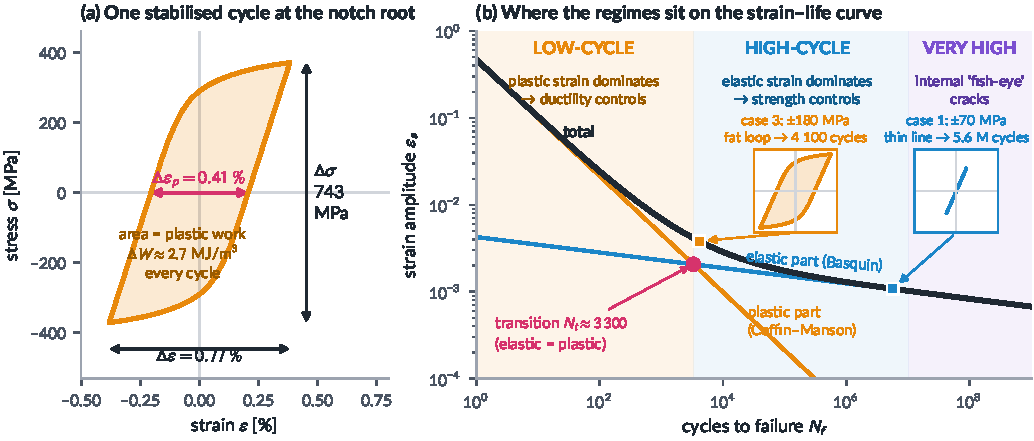
\includegraphics[width=\linewidth]{figs/fig01_overview.pdf}
\caption{(a) Stabilised loop at the hole of the FE plate (case 3, $\pm180$\,MPa): 0.41\,\% plastic strain range, 2.7\,MJ/m$^3$ dissipated per cycle. (b) The strain–life curve splits into an \elastic{elastic} and a \plastic{plastic} part. Where they cross (3\,300 cycles for this steel) LCF turns into HCF. The two insets use the same scale: a fat loop means LCF, a thin line means HCF.}
\label{fig:overview}
\end{figure}

The total strain amplitude is the sum of an elastic (strength) part and a plastic (ductility) part. This is the \textbf{Coffin–\allowbreak Manson–\allowbreak Basquin} relation; with the S355-type parameters used throughout:
\begin{equation*}
\varepsilon_a=\underbrace{\elastic{\frac{\sigma_f'}{E}\,(2N_f)^{b}}}_{\text{elastic: strength}}+\underbrace{\plastic{\varepsilon_f'\,(2N_f)^{c}}}_{\text{plastic: ductility}}
\;=\;\elastic{\frac{952}{210\,000}\,(2N_f)^{-0.089}}+\plastic{0.737\,(2N_f)^{-0.668}} .
\end{equation*}
The \textbf{transition life} is where both parts are equal:
\begin{equation*}
2N_t=\left(\frac{\varepsilon_f'E}{\sigma_f'}\right)^{\frac{1}{b-c}}=\left(\frac{0.737\cdot210\,000}{952}\right)^{\frac{1}{0.579}}\approx 6\,600\ \text{reversals}
\;\Rightarrow\; N_t\approx3\,300\ \text{cycles}.
\end{equation*}
Low-strength, ductile steels have long transition lives; high-strength steels reach it after a few hundred cycles. Beyond about $10^7$ cycles (very-high-cycle fatigue) cracks start inside the material at inclusions ("fish-eyes"), so a true fatigue limit is no longer assumed.

\begin{keybox}[corange]{Why notches matter.}
In a real part the bulk stays elastic while the notch root yields. The elastic surroundings then \emph{impose a strain cycle} on the notch. That is why local strain methods and FE analysis sit at the centre of both regimes.
\end{keybox}

%-------------------------------------------------------------------------------- 2
\section{High-cycle fatigue: the stress–life toolbox}
\begin{figure}[h]
\centering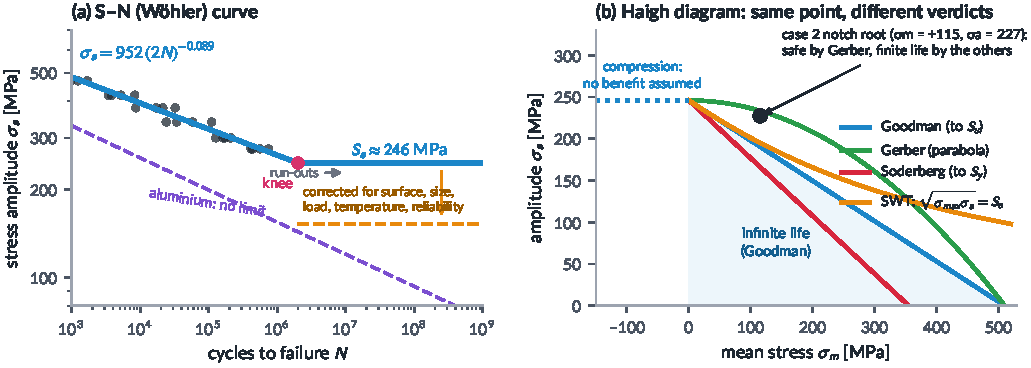
\includegraphics[width=\linewidth]{figs/fig02_hcf.pdf}
\caption{(a) The S–N curve: a straight line (Basquin) down to a knee, then a fatigue limit for steels. The limit is lowered for real surfaces, sizes and loading. (b) Mean-stress rules in the Haigh diagram. The notch-root point of FE case 2 passes Gerber but fails Goodman, Soderberg and SWT, so the choice of rule matters.}
\label{fig:hcf}
\end{figure}

\textbf{Basquin and the fatigue limit.} In the finite-life region,
\begin{equation*}
\sigma_a=\sigma_f'\,(2N)^{b}=952\,(2N)^{-0.089}\MPa
\quad\Rightarrow\quad S_e=\sigma_a(N=2\cdot10^6)=952\,(4\cdot10^{6})^{-0.089}\approx246\MPa .
\end{equation*}
For design, $S_e$ is reduced by factors for surface, size, load type, temperature and reliability: $S_e=k_ak_bk_ck_dk_e\,S_e'$.

\textbf{Mean stress} (Fig.~\ref{fig:hcf}b). Each rule converts $(\sigma_a,\sigma_m)$ into an equivalent fully reversed amplitude, to be compared with $S_e=246$\,MPa. For the notch root of case 2 ($\sigma_a=227$, $\sigma_m=115$, $\sigma_{\max}=343$\,MPa, $S_u=510$, $S_y=355$\,MPa):
\begin{numbox}
\vspace{-4pt}
\begin{align*}
\text{Goodman:}\ & \frac{\sigma_a}{1-\sigma_m/S_u}=\frac{227}{1-115/510}=294 &
\text{Gerber:}\ & \frac{\sigma_a}{1-(\sigma_m/S_u)^2}=\frac{227}{1-0.051}=240\\
\text{Soderberg:}\ & \frac{\sigma_a}{1-\sigma_m/S_y}=\frac{227}{1-115/355}=337 &
\text{SWT:}\ & \sqrt{\sigma_{\max}\sigma_a}=\sqrt{343\cdot227}=279\ \ \text{MPa}
\end{align*}
\end{numbox}
Only Gerber stays below 246\,MPa (infinite life). The others predict a finite life, from the same stresses.

\subsection{Notches: $K_t$ and $K_f$}
\begin{figure}[h]
\centering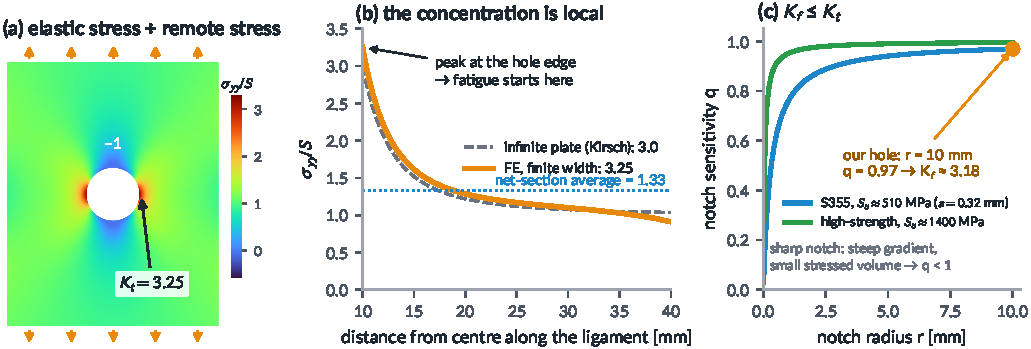
\includegraphics[width=\linewidth]{figs/fig03_notch.pdf}
\caption{(a) Elastic FE stress at the hole, normalised by the remote stress. (b) The peak of 3.25 decays within about one radius; equilibrium fixes the average at 1.33. (c) Notch sensitivity: sharp notches hurt less than $K_t$ suggests. A 10\,mm radius gives $q\approx0.97$, so $K_f\approx K_t$.}
\label{fig:notch}
\end{figure}
\begin{gather*}
K_t=\frac{\sigma_{\max}}{S}=\frac{227}{70}=3.25\quad\bigl(K_{t,\text{net}}=2.44,\ \text{Peterson: } 2.43\bigr)\\
K_f=1+q\,(K_t-1),\qquad q=\frac{1}{1+a/r}=\frac{1}{1+0.32/10}=0.97\ \ \Rightarrow\ \ K_f=1+0.97\,(3.25-1)\approx3.18
\end{gather*}

\subsection{Welded joints: three routes to the same answer}
The weld toe is a sharp notch with residual stress near yield. Weld S–N curves therefore largely \emph{ignore applied mean stress} and are given for stress \emph{ranges} $\Delta\sigma$.
\begin{figure}[h]
\centering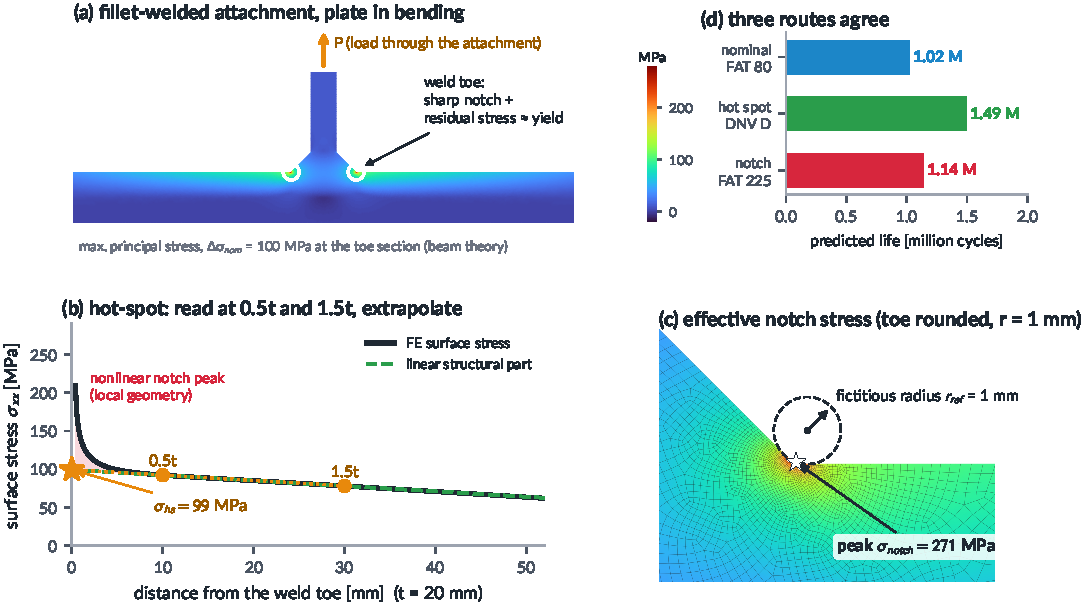
\includegraphics[width=\linewidth]{figs/fig04_weld.pdf}
\caption{(a) FE model of a fillet-welded attachment, with the plate in bending. (b) The surface stress is a linear \emph{structural} part plus a sharp \emph{notch peak}. The hot-spot method reads the structural part at $0.5t$ and $1.5t$ and extrapolates to the toe. (c) The effective notch method rounds the toe with $r_{ref}=1$\,mm and uses the peak directly. (d) All three routes give 1.0–1.5 million cycles.}
\label{fig:weld}
\end{figure}
\begin{numbox}
\vspace{-4pt}
\begin{align*}
\textbf{nominal (FAT 80):}\quad & N=2\cdot10^{6}\Bigl(\frac{80}{100}\Bigr)^{3}=1.02\cdot10^{6}\\
\textbf{hot spot (DNV-RP-C203):}\quad & \sigma_{hs}=1.5\,\sigma_{0.5t}-0.5\,\sigma_{1.5t}=1.5(92.2)-0.5(78.1)=99.2\MPa\\
& N=\frac{10^{12.164}}{\Delta\sigma_{hs}^{3}}=\frac{10^{12.164}}{99.2^{3}}=1.49\cdot10^{6}\ \text{(curve D)}\\
\textbf{effective notch (IIW):}\quad & \sigma_{notch}=271\MPa,\quad N=2\cdot10^{6}\Bigl(\frac{225}{271}\Bigr)^{3}=1.14\cdot10^{6}\ \text{(FAT 225)}
\end{align*}
\end{numbox}
Each route only works if its own meshing and read-out rules are followed exactly.

\subsection{Variable amplitude: rainflow counting and Miner's rule}
\begin{figure}[h]
\centering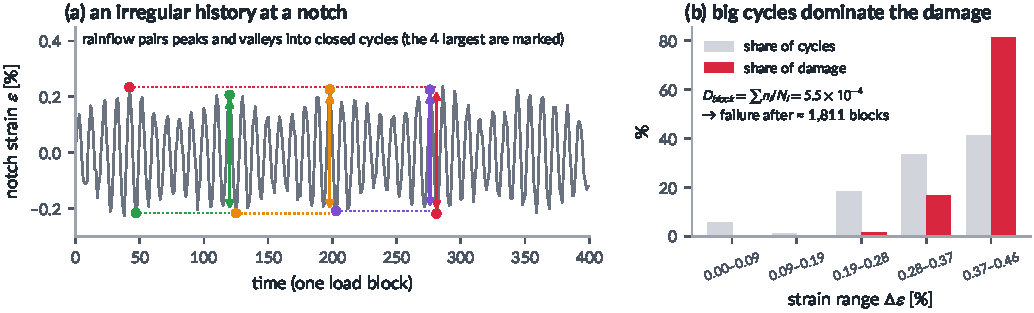
\includegraphics[width=\linewidth]{figs/fig05_rainflow.pdf}
\caption{(a) Rainflow counting extracts closed cycles from an irregular history. (b) Life falls steeply with range, so damage is concentrated in the big cycles. The largest 20\,\% of the cycles cause about half of the damage, and the smallest quarter (ranges below 0.28\,\%) cause less than 2\,\%.}
\label{fig:rain}
\end{figure}
Each counted cycle uses up the fraction $n_i/N_i$ of the life at its range, and the \textbf{Palmgren–Miner} rule adds the fractions:
\begin{equation*}
D=\sum_i\frac{n_i}{N_i}\le 1\ \ \Bigl(\text{design: }D\le\tfrac{1}{\text{DFF}}\Bigr),\qquad
\text{Fig.~\ref{fig:rain}: } D_{\text{block}}=5.5\cdot10^{-4}\ \Rightarrow\ \approx1\,800\ \text{blocks to failure}.
\end{equation*}
Miner ignores load sequence. Multiaxial stress needs invariant criteria (Sines, Crossland), mesoscopic ones (Dang Van) or critical-plane criteria (Findley).

%-------------------------------------------------------------------------------- 3
\section{Low-cycle fatigue: the strain–life toolbox}
Under cyclic straining, metals harden (soft, annealed) or soften (cold-worked, high-strength) until the loops stabilise. The tips of the stable loops define the \textbf{cyclic stress–strain curve}. With \textbf{Masing} behaviour each loop branch is that curve scaled by two (Fig.~\ref{fig:lcf}a):
\begin{equation*}
\varepsilon_a=\frac{\sigma_a}{E}+\Bigl(\frac{\sigma_a}{K'}\Bigr)^{1/n'}=\frac{\sigma_a}{210\,000}+\Bigl(\frac{\sigma_a}{596}\Bigr)^{1/0.076},\qquad
\frac{\Delta\varepsilon}{2}=\frac{\Delta\sigma}{2E}+\Bigl(\frac{\Delta\sigma}{2K'}\Bigr)^{1/n'} .
\end{equation*}

\begin{figure}[h]
\centering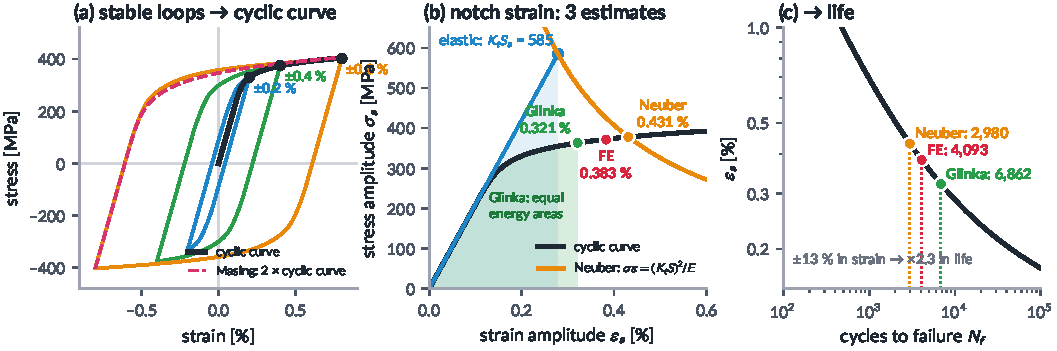
\includegraphics[width=\linewidth]{figs/fig06_lcf.pdf}
\caption{(a) Stable loops at three strain amplitudes. Their tips form the cyclic curve, and the dashed Masing branch (twice the cyclic curve) matches the loop. (b) Notch-root strain from Neuber's hyperbola, Glinka's equal-energy rule and elastic-plastic FE. (c) A 13\,\% difference in strain changes the predicted life by a factor of 2.3.}
\label{fig:lcf}
\end{figure}

\textbf{Notch strain} for case 3 ($S_a=180$\,MPa, so the elastic notch stress is $K_tS_a=585$\,MPa):
\begin{numbox}
\vspace{-4pt}
\begin{align*}
\textbf{Neuber:}\quad & \sigma_a\varepsilon_a=\frac{(K_tS_a)^2}{E}=\frac{585^2}{210\,000}=1.63\MPa &&\Rightarrow\ \varepsilon_a=0.431\,\%,\ N_f\approx2\,980\\
\textbf{Glinka:}\quad & \int_0^{\varepsilon_a}\!\sigma\,d\varepsilon=\frac{(K_tS_a)^2}{2E}=0.81\MPa &&\Rightarrow\ \varepsilon_a=0.321\,\%,\ N_f\approx6\,860\\
\textbf{FE (Chaboche):}\quad & \text{stabilised loop at the hole} &&\Rightarrow\ \varepsilon_a=0.383\,\%,\ N_f\approx4\,100
\end{align*}
\end{numbox}
Neuber overestimates the strain and Glinka underestimates it. FE lies in between.

\textbf{Mean stress in strain–life.} Morrow subtracts the mean stress from the strength term; Smith–Watson–Topper uses the peak stress:
\begin{equation*}
\varepsilon_a=\frac{\sigma_f'-\sigma_m}{E}(2N_f)^{b}+\varepsilon_f'(2N_f)^{c},\qquad
\sigma_{\max}\,\varepsilon_a=\frac{(\sigma_f')^2}{E}(2N_f)^{2b}+\sigma_f'\varepsilon_f'(2N_f)^{b+c}.
\end{equation*}
For the case-2 notch root ($\varepsilon_a=0.108$\,\%, $\sigma_m=+115$\,MPa) the predicted life drops from $5.6\cdot10^6$ cycles (no mean stress) to $1.6\cdot10^6$ (Morrow) and $0.63\cdot10^6$ (SWT).

\textbf{In design codes.} ASME VIII-2 offers an elastic route, where the stress range is amplified by $K_e\ge1$ above the shakedown limit, and an elastic-plastic route with $\Delta\varepsilon_{eff}=\Delta S_P/E+\Delta\varepsilon_{peq}$ from a cyclic analysis. DNV-RP-C203 corrects elastic hot-spot ranges for plasticity in LCF and sums $D=D_{LCF}+D_{HCF}$.

%-------------------------------------------------------------------------------- 4
\section{Finite element study: one plate, four regimes}
\begin{figure}[h]
\centering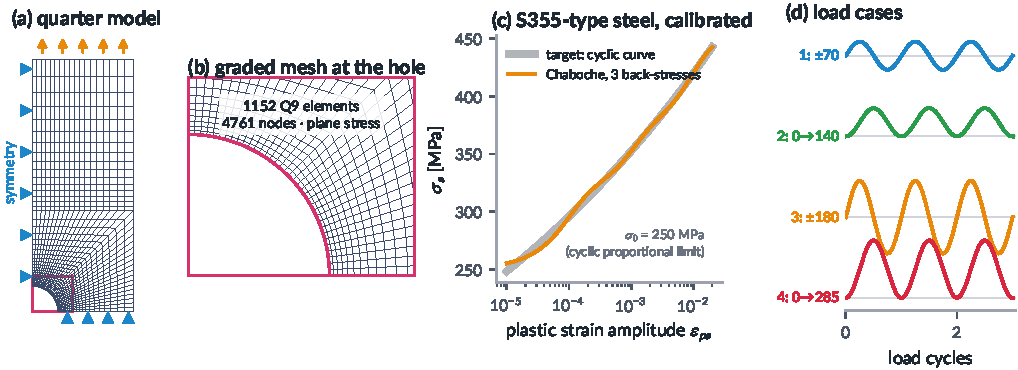
\includegraphics[width=\linewidth]{figs/fig07_model.pdf}
\caption{(a–b) Quarter model of an 80\,mm wide plate with a $\varnothing$20\,mm hole: plane stress, 1152 nine-node elements graded towards the hole. (c) S355-type steel: three Chaboche back-stresses fitted to the cyclic curve. (d) The four load cases.}
\label{fig:model}
\end{figure}
The material uses nonlinear kinematic (Chaboche) hardening. Each back-stress grows with plastic flow and saturates:
\begin{equation*}
d\boldsymbol{\alpha}_i=\tfrac{2}{3}C_i\,d\boldsymbol{\varepsilon}_p-\gamma_i\,\boldsymbol{\alpha}_i\,dp
\quad\Rightarrow\quad
\sigma_a=\sigma_0+\sum_i\frac{C_i}{\gamma_i}\tanh(\gamma_i\varepsilon_{pa})
\end{equation*}
\vspace{-2pt}
\begin{equation*}
\sigma_a=250+60.6\tanh(8000\,\varepsilon_{pa})+53.0\tanh(800\,\varepsilon_{pa})+85.5\tanh(80\,\varepsilon_{pa})\ \ \text{MPa}
\end{equation*}
\vspace{-6pt}
\begin{center}\small
\begin{tabular}{lcc}
\toprule
\textbf{verification} & \textbf{in-house solver} & \textbf{reference} \\
\midrule
elastic $K_{t,\text{net}}$, $d/W=0.25$ & 2.437 & 2.43 (Peterson) \\
notch strain at $S=+220$\,MPa, elastic–perfectly plastic & 0.597\,\% & 0.604\,\% (CalculiX) \\
PEEQ after one cycle (same model) & 2.14\,\% & 2.18\,\% (CalculiX) \\
Bree diagram, 6\,561 load points & 6\,560 match & Bree (1967) theory \\
\bottomrule
\end{tabular}
\end{center}

\begin{figure}[tb]
\centering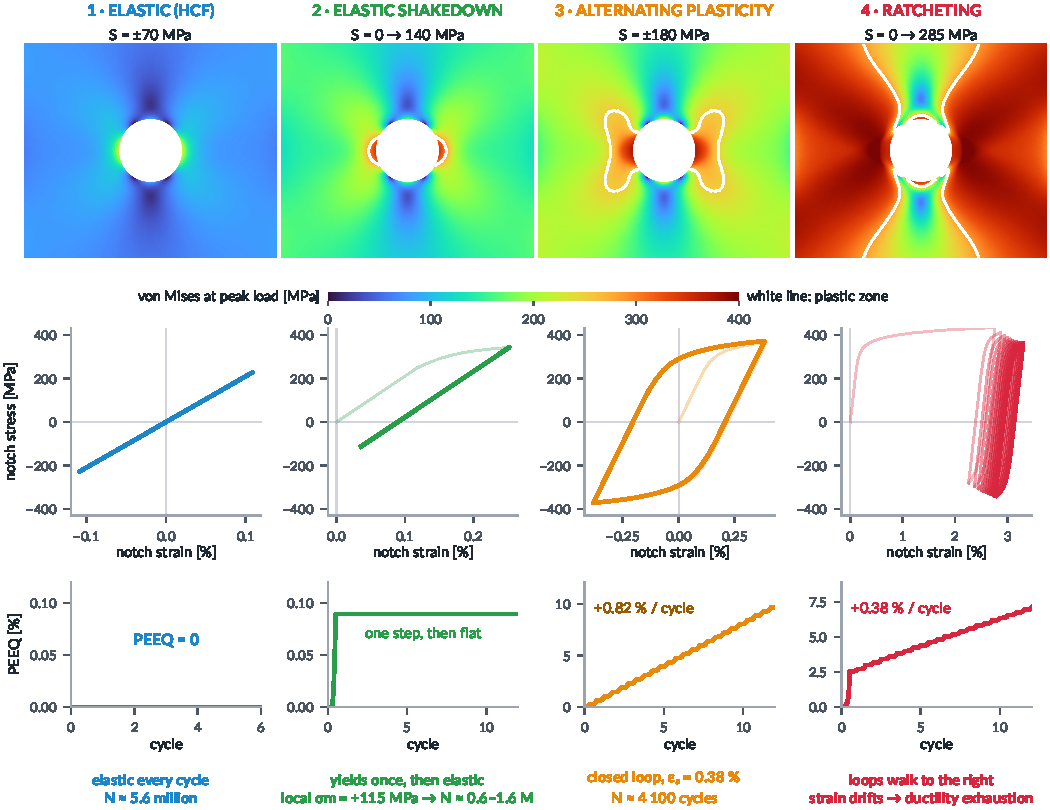
\includegraphics[width=\linewidth]{figs/fig08_regimes.pdf}
\caption{\textbf{The four possible responses, from the same plate.} Top: von Mises stress at peak load, with the plastic zone outlined in white. Middle: stress–strain at the hole edge over all cycles (darker = later). Bottom: accumulated plastic strain (PEEQ) at the hole edge. (1) elastic: a line, no PEEQ. (2) yields once, then purely elastic (shakedown), but with a +115\,MPa residual mean stress. (3) closed loop every cycle (LCF). (4) the net section yields and the loop walks: ratcheting. Cases 3 and 4 both show rising PEEQ but are entirely different problems.}
\label{fig:regimes}
\end{figure}

Why each case behaves as it does follows from the \textbf{shakedown condition}: the elastic stress range must fit inside the elastic domain, which is $2\sigma_0=500$\,MPa wide for this material:
\begin{gather*}
\text{case 2: }\ \Delta\sigma_{el}=K_t\,\Delta S=3.25\cdot140=455\MPa<500\MPa\ \Rightarrow\ \text{\textcolor{cgreen}{elastic shakedown}}\\
\text{case 3: }\ \Delta\sigma_{el}=3.25\cdot360=1170\MPa>500\MPa\ \Rightarrow\ \text{\textcolor{corange}{plastic flow every cycle}}
\end{gather*}

\begin{center}\small
\begin{tabularx}{\linewidth}{l l X l}
\toprule
\textbf{case} & \textbf{remote stress} & \textbf{hole-edge response (stabilised)} & \textbf{life} \\
\midrule
\textcolor{cblue}{1 elastic} & $\pm70$\,MPa & elastic, $\sigma_a=227<S_e$, PEEQ $=0$ & $5.6\cdot10^{6}$ \\
\textcolor{cgreen}{2 shakedown} & $0\to140$\,MPa & yields once, then elastic; local $\sigma_m=+115$\,MPa & $0.6$–$1.6\cdot10^{6}$ \\
\textcolor{corange}{3 alternating} & $\pm180$\,MPa & closed loop, $\varepsilon_a=0.383\,\%$, PEEQ $+0.82\,\%$/cycle & $\approx4\,100$ \\
\textcolor{cred}{4 ratcheting} & $0\to285$\,MPa & loops walk, mean strain $\approx3\,\%$ and growing & ductility exhaustion \\
\bottomrule
\end{tabularx}
\end{center}

%-------------------------------------------------------------------------------- 5
\section{Accumulated plastic strain: what it is, and when it is a problem}
\begin{minipage}[t]{0.50\linewidth}
\vspace{0pt}
Most FE codes report the \textbf{equivalent plastic strain} (PEEQ in Abaqus):
\begin{equation*}
\bar\varepsilon_p=\int_0^t\sqrt{\tfrac{2}{3}\,\dot{\boldsymbol\varepsilon}_p:\dot{\boldsymbol\varepsilon}_p}\;dt\ \ \ge0 .
\end{equation*}
It integrates the \emph{magnitude} of plastic flow, so every reversal adds to it, in any direction. In uniaxial alternating plasticity it grows by twice the plastic strain range per cycle:
\begin{equation*}
\Delta\bar\varepsilon_p^{\,\text{cycle}}=2\,\Delta\varepsilon_p=2\times0.41\,\%=0.82\,\%,
\end{equation*}
while the strain itself only oscillates between $\pm0.38$\,\% (Fig.~\ref{fig:peeq}). A large PEEQ alone therefore does not tell you whether you have a fatigue problem, a ratcheting problem or neither. Instead, look at the \textbf{change of the plastic strain tensor over a full cycle}:
\begin{equation*}
\Delta\boldsymbol\varepsilon_p^{\text{cycle}}=\boldsymbol\varepsilon_p(t_N)-\boldsymbol\varepsilon_p(t_{N-1})
\begin{cases}\approx\mathbf 0 & \text{no ratcheting}\\ \neq\mathbf 0 & \text{ratcheting}\end{cases}
\end{equation*}
\end{minipage}\hfill
\begin{minipage}[t]{0.47\linewidth}
\vspace{2pt}
\centering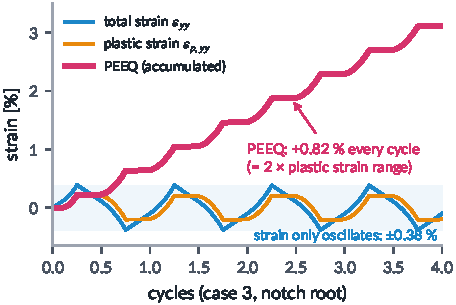
\includegraphics[width=\linewidth]{figs/fig09_peeq.pdf}
\captionof{figure}{PEEQ climbs like a staircase although the strain at the notch just cycles (case 3).}
\label{fig:peeq}
\end{minipage}

\subsection{Shakedown, alternating plasticity and ratcheting}
\textbf{Melan's theorem}: if \emph{some} constant, self-equilibrating residual stress field $\boldsymbol\rho$ keeps the elastic stresses plus $\boldsymbol\rho$ inside the yield surface at all times, the structure shakes down (Fig.~\ref{fig:bree}a). For an elastic–perfectly plastic material this gives $\Delta\sigma_{eq}^{el}\le2\sigma_y$, the basis of the ASME limit $S_{PS}=\max(3S,\,2S_y)$ on the primary-plus-secondary stress range.

Ratcheting needs a \textbf{sustained primary load} plus a \textbf{cyclic secondary stress}. In the classic \textbf{Bree problem}, a pressurised tube is cycled with a through-wall temperature difference, with $X=\sigma_{\text{primary}}/\sigma_y$ and $Y=\sigma_{\text{thermal}}/\sigma_y$:
\begin{equation*}
\text{elastic: }X+Y\le1,\qquad
\text{alternating plasticity: }Y>2,\ XY\le1,\qquad
\text{ratcheting: }\ \underbrace{X+\tfrac{Y}{4}>1}_{Y\le2\ (R_1)}\ \ \text{or}\ \ \underbrace{XY>1}_{Y>2\ (R_2)} .
\end{equation*}
\begin{figure}[h]
\centering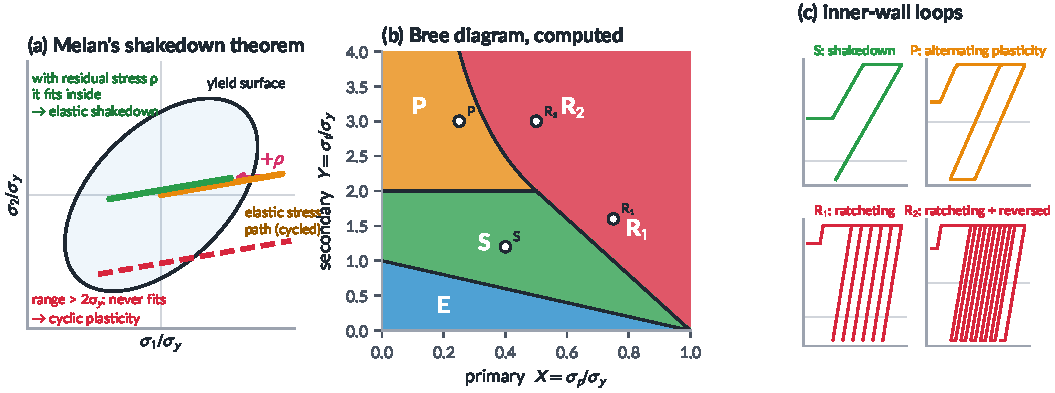
\includegraphics[width=\linewidth]{figs/fig10_bree.pdf}
\caption{(a) Melan: a residual stress can shift an elastic stress path inside the yield surface. A range above $2\sigma_y$ never fits. (b) The Bree diagram computed with a through-wall FE fibre model (6\,561 load cases, 24 cycles each) reproduces Bree's analytical lines at all but one point, which sits exactly on a boundary. (c) Inner-wall loops: a line after the first cycle (S), a closed loop (P), loops that walk (R$_1$, R$_2$).}
\label{fig:bree}
\end{figure}

\begin{figure}[h]
\centering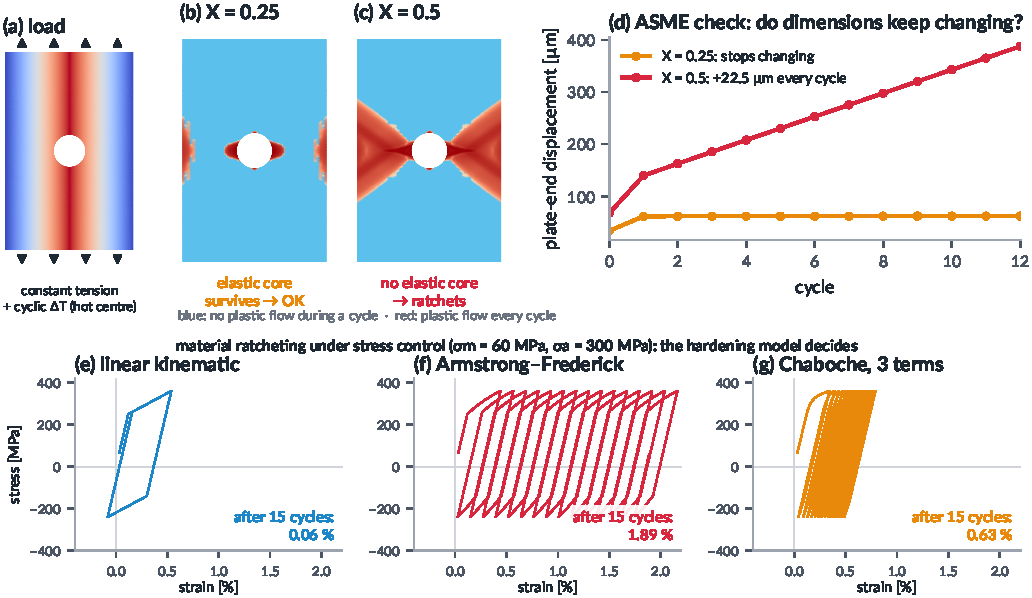
\includegraphics[width=\linewidth]{figs/fig11_ratchet.pdf}
\caption{Two kinds of ratcheting. Top, \emph{structural}: the holed plate under constant tension and a cycled temperature field (elastic–perfectly plastic, as codes require). At $X=0.25$ an elastic core (blue) survives each cycle and the length stops changing. At $X=0.5$ the whole ligament yields every cycle and the plate grows 22.5\,µm per cycle, the Bree logic again ($XY=1.25>1$). Bottom, \emph{material}: under stress control with a mean stress the predicted ratcheting depends entirely on the hardening model.}
\label{fig:ratchet}
\end{figure}

\subsection{How to assess it in practice}
\begin{enumerate}[leftmargin=14pt]
\item \textbf{Run enough cycles}: at least 3 (ASME VIII-2). Eurocode 3-1-6 uses the strain increment after the 3rd cycle.
\item \textbf{Separate the response}: the net plastic strain per cycle shows ratcheting, the plastic strain range shows LCF, and the change of key dimensions per cycle shows structural ratcheting.
\item \textbf{Apply the acceptance criteria:}
\end{enumerate}
\vspace{-2pt}
{\small
\begin{tabularx}{\linewidth}{>{\bfseries}p{3.7cm} X}
\toprule
ASME VIII-2, ratcheting & elastic–perfectly plastic model, $\ge3$ cycles. Passes if \emph{one} holds: (a) no plastic action, (b) an elastic core in the primary-load-bearing boundary, (c) no permanent change in overall dimensions. \\ \addlinespace[3pt]
EN 13445-3, Annex B & progressive-deformation check: shakedown must be shown, e.g.\ with Melan's theorem. \\ \addlinespace[3pt]
EN 1993-1-6, LS2 & $\varepsilon_{p,eq,Ed}\le25\,f_y/E=25\cdot355/210\,000=4.2\,\%$ over the design life, with $\varepsilon_{p,eq,Ed}\approx n_{cyc}\,\Delta\varepsilon_{p,eq}$. \\ \addlinespace[3pt]
ASME VIII-2, local failure & $\varepsilon_{peq}+\varepsilon_{cf}\le\varepsilon_L=\varepsilon_{Lu}\exp\!\bigl[-\tfrac{\alpha_{sl}}{1+m_2}\bigl(\tfrac{\sigma_1+\sigma_2+\sigma_3}{3\sigma_e}-\tfrac13\bigr)\bigr]$: high triaxiality lowers the allowable strain. For load sequences, $D_\varepsilon=\sum\Delta\varepsilon_{peq,k}/\varepsilon_{L,k}\le1$. \\
\bottomrule
\end{tabularx}}
\vspace{2pt}
\begin{enumerate}[leftmargin=14pt,resume]
\item \textbf{Add up the damage.} For alternating plasticity, take LCF from the stabilised strain range and add it to HCF. If ratcheting persists, ductility is consumed on top of fatigue:
\begin{equation*}
D=D_{LCF}\bigl(\Delta\varepsilon_{\text{stabilised}}\bigr)+D_{HCF}\le1,\qquad\qquad
D=D_{\text{fatigue}}+\underbrace{\frac{\varepsilon_{\text{ratchet}}}{\varepsilon_f}}_{\text{ductility used up}}
\end{equation*}
Design codes generally do not accept ratcheting that continues.
\end{enumerate}

%-------------------------------------------------------------------------------- 6
\section{Putting it together}
\begin{center}
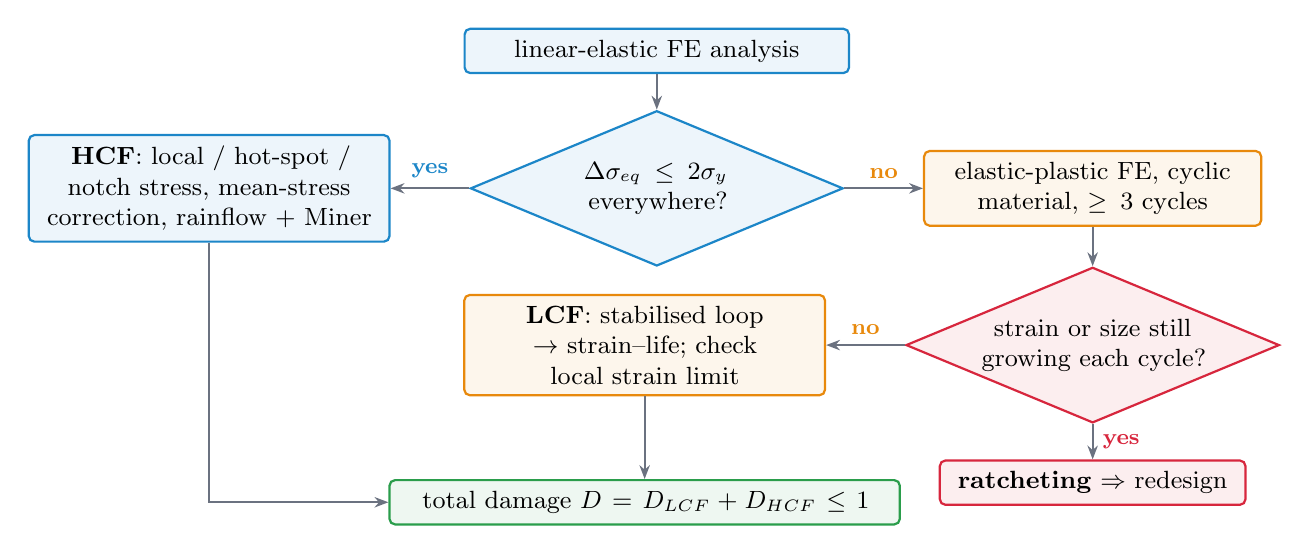
\begin{tikzpicture}[
  node distance=0.45cm and 0.9cm, font=\small,
  box/.style={rectangle,rounded corners=2pt,draw=#1,fill=#1!8,line width=0.8pt,align=center,inner sep=4pt,text width=4.6cm},
  dec/.style={diamond,aspect=2.4,draw=#1,fill=#1!8,line width=0.8pt,align=center,inner sep=1pt,text width=2.9cm},
  arr/.style={-{Stealth[length=5pt]},line width=0.8pt,draw=cgray}]
\node[box=cblue] (a) {linear-elastic FE analysis};
\node[dec=cblue,below=of a] (b) {$\Delta\sigma_{eq}\le2\sigma_y$\\ everywhere?};
\node[box=cblue,left=1.0cm of b,text width=4.3cm] (c) {\textbf{HCF}: local / hot-spot / notch stress, mean-stress correction, rainflow + Miner};
\node[box=corange,right=1.0cm of b,text width=4.0cm] (d) {elastic-plastic FE, cyclic material, $\ge3$ cycles};
\node[dec=cred,below=0.5cm of d] (e) {strain or size still\\ growing each cycle?};
\node[box=cred,below=0.45cm of e,text width=3.6cm] (f) {\textbf{ratcheting} $\Rightarrow$ redesign};
\node[box=corange,left=1.0cm of e,text width=4.3cm] (g) {\textbf{LCF}: stabilised loop $\to$ strain–life; check local strain limit};
\node[box=cgreen,below=1.05cm of g,text width=6.2cm] (h) {total damage $D=D_{LCF}+D_{HCF}\le1$};
\draw[arr] (a) -- (b);
\draw[arr] (b) -- node[above,font=\footnotesize\bfseries,text=cblue]{yes} (c);
\draw[arr] (b) -- node[above,font=\footnotesize\bfseries,text=corange]{no} (d);
\draw[arr] (d) -- (e);
\draw[arr] (e) -- node[right,font=\footnotesize\bfseries,text=cred]{yes} (f);
\draw[arr] (e) -- node[above,font=\footnotesize\bfseries,text=corange]{no} (g);
\draw[arr] (c.south) |- (h.west);
\draw[arr] (g.south) -- (h.north -| g.south);
\end{tikzpicture}
\end{center}
\vspace{-4pt}
\begin{keybox}[cgreen]{Bottom line.}
\textbf{HCF} is governed by stress amplitude and strength, \textbf{LCF} by plastic strain range and ductility. \textbf{Accumulated plastic strain} only means something once you know whether it stopped (shakedown), cycles (LCF) or drifts (ratcheting).
\end{keybox}

{\footnotesize\color{cgray}
\textbf{Notes.} Material data are representative S355 values, used for illustration; use test data in design. Code clauses are summarised for orientation; apply the governing edition and national annexes.
\textbf{Further reading.} N.E.~Dowling, \emph{Mechanical Behavior of Materials}; R.I.~Stephens et al., \emph{Metal Fatigue in Engineering}; A.~Hobbacher, \emph{IIW Recommendations for Fatigue Design of Welded Joints}; DNV-RP-C203 \emph{Fatigue design of offshore steel structures}; ASME BPVC VIII-2, Part 5; EN 13445-3, Annex B; EN 1993-1-6; J.~Bree (1967) \emph{J.\ Strain Anal.} 2:226; J.L.~Chaboche (1989) \emph{Int.\ J.\ Plasticity} 5:247; H.~Neuber (1961) \emph{J.\ Appl.\ Mech.} 28:544; G.~Glinka (1985) \emph{Eng.\ Fract.\ Mech.} 22:485.\par}

\end{document}
